\documentclass{uestcMath}
\def\currentvolume{*}
\def\currentissue{*}
\def\currentyear{*}
\def\currentmonth{*}
\def\doi{10.11948/\currentyear***}
\firstpage{1}
%%%%%%%%%%%%%%%%%%%%%%%%%%%%%%%%%%%%%%  The above is inserted by publisher. %%%%%%%%%%%%%%%%%%%%%%

%%%%%%%%%%%%%%%%%%%%%%   The following packages have been used in this template. %%%%%%%%%%%%%%%%%%
%\usepackage{amsmath}
%\usepackage{amsthm}
%\usepackage{amssymb}
%\usepackage{graphicx}
%\usepackage{cite}
%\usepackage{epsfig}
%\usepackage[normal]{subfigure}
%\usepackage{paralist}
%\usepackage{caption2}
%\usepackage{hyperref}
%%%%%%%%%%%%%%%%%%%%%%%  Please state your own packages below. %%%%%%%%%%%%%%%%%%%%%%%%%%%%%%%%
%\usepackage{}
%\usepackage{}
%\usepackage{}
%\graphicspath{{figures/}}
%%%%%%%%%%%%%%%%%%%%%%%%%%%%%%%%%%%%%%%%%%%%%%%%%%%%%%%%%%%%%%%%%%%%%%%%%%%%%%%%%%%%%%%%%%%%%%%%
%%%%%%%%%%%%%%%%%%%%%%%%          The following are editted        %%%%%%%%%%%%%%%%%%%%%%%%%%%%%
%%%%%%%%%%%%%%%%%%%%%%%%               by the author.              %%%%%%%%%%%%%%%%%%%%%%%%%%%%%
%%%%%%%%%%%%%%%%%%%%%%%%%%%%%%%%%%%%%%%%%%%%%%%%%%%%%%%%%%%%%%%%%%%%%%%%%%%%%%%%%%%%%%%%%%%%%%%%

\def\shorttitle{The shorttitle of your paper. It is up to 40 characters}


\def\shortauthor{A. Author,  B. Author \& C. Author}


\title{Please use pdflatex to run your paper$^*$}

\author{ A** Author$^{1,\dag}$, B** Author$^2$ and C** Author$^2$}%%%%%%%%  Here is the full name of every author. %%%%%%%%%%%%%%%%%%

\date{}


\begin{document}
\baselineskip 12pt

\maketitle
\begin{abstract}
Here is the  content of your abstract. It should not contain any displayed equations.
\end{abstract}

\begin{keyword}
A list of 3-5 keywords are to be supplied. (Use semicolon ``;" to separate each one and capitalize the first letter of the first word only.)
\end{keyword}

\begin{MSC}
**; **.
(This is the 2010 Mathematics Subject Classification of your paper. Use semicolon ``;" to separate each one.)
\end{MSC}


\thispagestyle{first}\renewcommand{\thefootnote}{\fnsymbol{footnote}}
\footnotetext{\hspace*{-5mm}
\renewcommand{\arraystretch}{1}
\begin{tabular}{@{}r@{}p{10cm}@{}}
$^\dag$& the corresponding author. Email address:***@***.**(A. Author)\\
$^1$&Department, University, Street, Postal-Code City, Country\\
$^2$&Laboratory, Institute, Street, Postal-Code City, Country\\
$^*$& The authors were supported by National Natural Science
Foundation of China (****) and National Science Foundation of
Shanghai (*****).
\end{tabular}}

\vspace{-2mm}


\section{Introduction}
Please prepare your tex file according to the following introduction
very closely. You need to check your manuscript carefully before you submit it. Thank you.



\section{The example of inserting a figure}
\begin{figure}[h!]
\centering
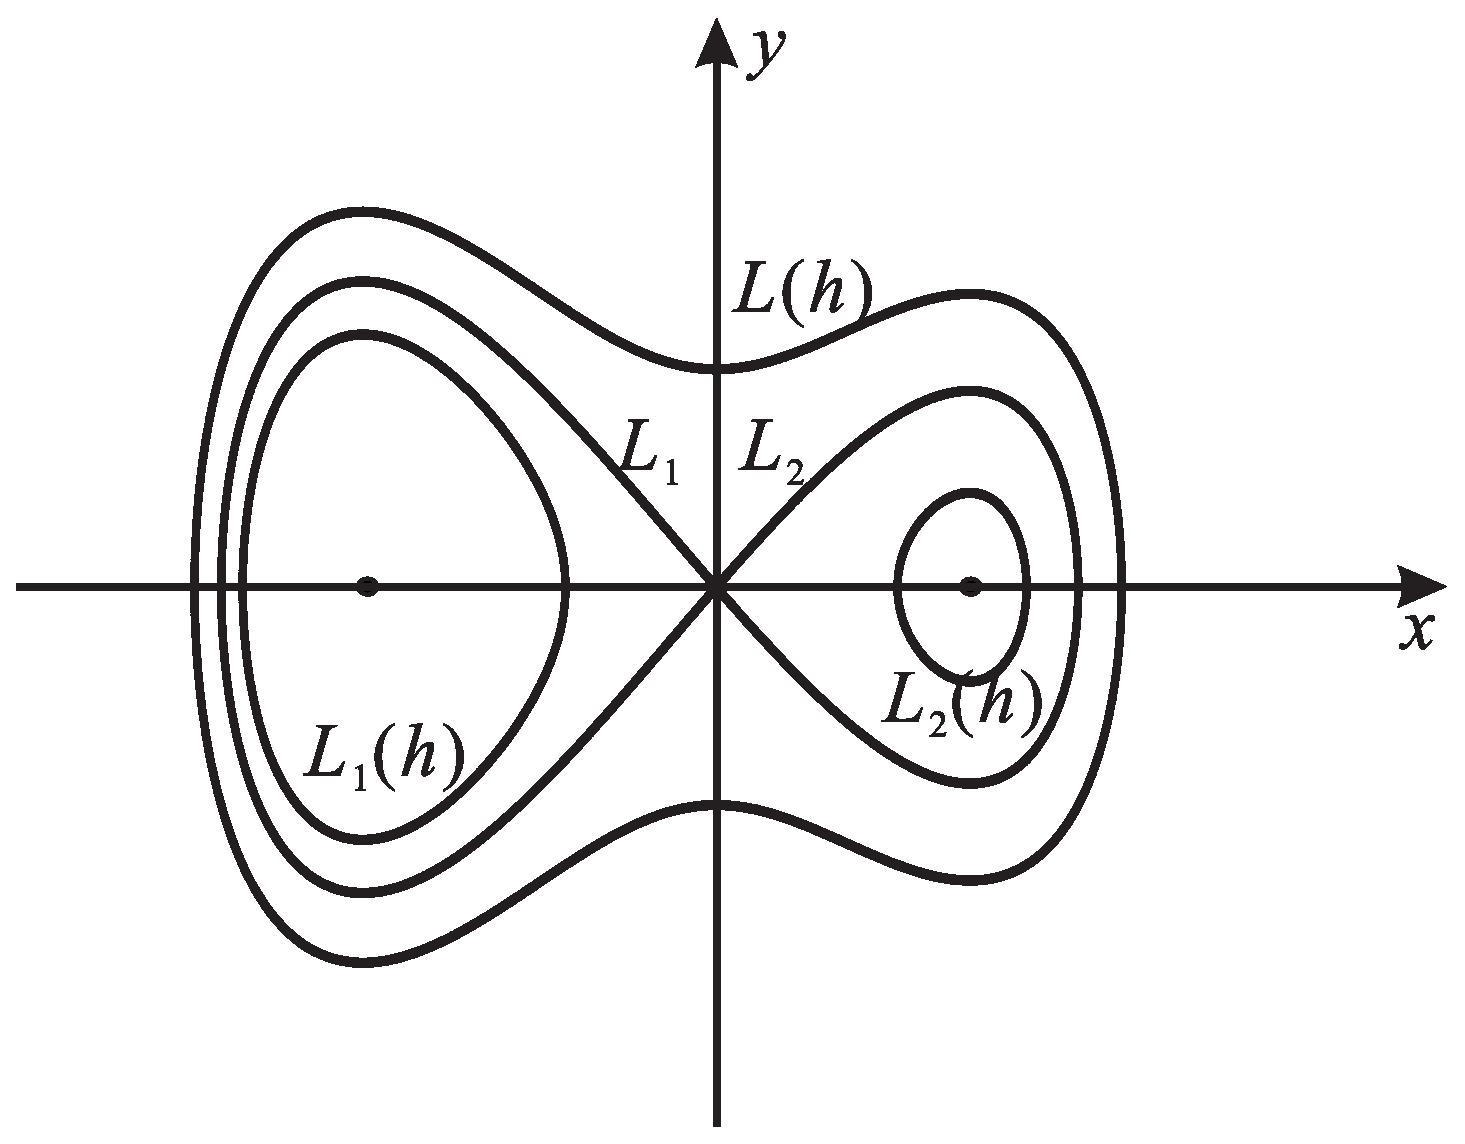
\includegraphics[scale=0.3]{fig1.eps}
\caption {The caption of your figure.}\label{fig1}
\end{figure}


\section{The  format of Theorem, Lemma, Proof and etc.}
\subsection{Theorem and Lemma}
 \noindent{\bf Input:}
\begin{verbatim}
\begin{theorem}\label{th1}
 Please state your theorem here.
 \end{theorem}
% `th1' is the label name of this theorem.
 \end{verbatim}

 \noindent{\bf Output:}
 \begin{theorem}\label{th1}
Please state your theorem here.
\end{theorem}

\noindent{\bf Input:}
\begin{verbatim}
\begin{lemma}[Lemma 2, \cite{ll2012}]\label{le1}
 Please state your lemma here. The format of item is as follows:
\begin{itemize}
\item[(i)] the first item;
\item[(ii)] the second item.
\end{itemize}
\end{lemma}
 \end{verbatim}

 \noindent{\bf Output:}
 \begin{lemma}[Lemma 2, \cite{ll2012}]
 \label{le1}
  Please state your lemma here. The format of item is as follows:
\begin{itemize}
\item[(i)] the first item;
\item[(ii)] the second item.
\end{itemize}
\end{lemma}

 \subsection{Proof}
\noindent{\bf Input:}

\begin{verbatim}
\begin{proof}
Please state your proof here.
\end{proof}
 \end{verbatim}

 \noindent{\bf Output:}

\begin{proof}
Please state your proof here.
\end{proof}


\subsection{The format of Definition, Remark,  Corollary and Example}
\begin{definition}\label{de1} Please state your definition here.\end{definition}

\begin{remark}\label{re1} Content of your remark.\end{remark}

\begin{corollary}\label{co1}Content of your corollary.\end{corollary}

\begin{example}\label{ex1}Content of your example.\end{example}




%%%%%%%%%%%%%%%%%%%%%%%%%%%%%%%%%   Here is the example of math formulas      %%%%%%%%%%%%%%%%%%%%%%%%%%%%%%%%%%%%%%%%%%

\section{The example of the math formulas}
Please align your math formulas as follows:
\begin{align*}
&\int_{\varepsilon_{0}}^{u_{0}(h)}\frac{u^{i}w^{j}}{u}du\\
=&\frac{h^{j}}{\lambda^{j}}\int_{\varepsilon_{0}}^{u_{0}}u^{i-j-1}du\vspace{.2cm}\\
=&\frac{1}{(i-j)\lambda^{j}}\Big[\,u_{0}^{i}\big(\frac{h}{u_{0}}\big)^{j}-\varepsilon_{0}^{i-j}h^{j}\,\Big] \vspace{.2cm}\\
\in& C^{\omega}.
\end{align*}

%\noindent Another way to align it:
%\begin{equation}\label{eq1}
%\begin{split}
%\int_{\varepsilon_{0}}^{u_{0}(h)}\frac{u^{i}w^{j}}{u}du&=\frac{h^{j}}{\lambda^{j}}\int_{\varepsilon_{0}}^{u_{0}}u^{i-j-1}du\vspace{.2cm}\\
%&=\frac{1}{(i-j)\lambda^{j}}\Big[\,u_{0}^{i}\big(\frac{h}{u_{0}}\big)^{j}-\varepsilon_{0}^{i-j}h^{j}\,\Big] \vspace{.2cm}\\
%&\in C^{\omega}.
%\end{split}
%\end{equation}

Here is an example if the math expression exceeds one line:
\begin{align}
f(1)=&1 + a_1 + a_2 + a_4 \nonumber\\
=&1-\Big(s_e'(L)bs_0M + s_m(M)+s_m'(M)\Big)
+s_e'(L)bs_0M \Big(s_m(M)+s_m'(M)M\nonumber\\
&-s_0M\Big) - b s_0 s_ps_e(L)\Big(s_l(L)+s_l'(L)L\Big)
\end{align}

For more than one equation:
\begin{align}
&A_{11}(b)=-\frac{2}{3}-\frac{2}{9}b^2-\sqrt 2\left(\frac{\pi}{2}+\theta\right)\left(\frac{1}{3}b+\frac{2}{27}b^3\right),\nonumber\\
&A_{12}(b)=\frac{13}{18}b+\frac{5}{27}b^3+\sqrt2\left(\frac{\pi}{2}+\theta\right)\left(\frac{1}{4}+\frac{1}{3}b^2+\frac{5}{81}b^4\right),\nonumber\\
&A_{13}(b)=-\frac{8}{15}-\frac{23}{27}b^2-\frac{14}{81}b^4-\sqrt2\Big(\frac{\pi}{2}+\theta\Big)\Big(\frac{1}{2}b+\frac{10}{27}b^3+\frac{14}{243}b^5\Big).\label{eq1}
\end{align}





\section{How to cite theorem, lemma and equation in the paper}

You need to {\bf label} the theorem, lemma and equation of this article first. Then \\

An example of label: ~~~~~~~~~Theorem \ref{th1} is labeled as {\bf th1}. \\

Another example of label: ~~~The equation \eqref{eq1} is labeled as {\bf eq1}.


\section*{Acknowledgements}
We would like to thank you to typeset your article according the above style very closely in
advance.


\section*{The format of citation}
\noindent {\bf Input:}
\begin{verbatim}
An example of book citation is Han \cite{H2013}.
An example of article citation is Imran etc \cite[p11]{ss2012}
 (if more than two co-authors).
More citations: \cite{H2013,ss2012,jr2}
 (if more than two references)
 \end{verbatim}

\vskip 2mm
\noindent {\bf Output:}
\vskip 2mm
\noindent An example of book citation is Han \cite{H2013}. \\
An example of article citation is  Imran etc \cite[p. 11-13]{ss2012}
 (if more than two co-authors).\\
More citations: \cite{H2013,ss2012,ll2012} (if more than two references).

\section*{The format of references}
A complete list of references cited, arranged in alphabetical order according to the surname of the first
author, should be provided. The first and middle name are listed in abbreviation form.

\vskip 3mm
\noindent{\em Book reference:}
\vskip 2mm
\noindent [1] ~~name1 and name2,  {\em The Name of The Book}, Publisher, address, year.

\vskip 3mm
\noindent {\em Journal reference~(Capitalize the first letter of the first word of paper title only):}
\vskip 2mm
\noindent [2] ~~name1, name2 and name3, {\em The name of the paper}, the name of the Journal, Vol(Year)(No), firstpage--lastpage.\par
\vskip 2mm
 {\it or article without volume and nomuber:}\par
\vskip 2mm
\noindent [3] ~~name1, name2 and name3, {\em The name of the paper}, the name of the Journal, (Year). DOI: doi number.


\bibliographystyle{jaacbib}
\bibliography{bibsample}% Here is the name of your BibTex database file.

%% Authors are advised to use a BibTeX database file for their reference list.
%% It can also be listed in the main tex file as follows:

\begin{thebibliography}{99}
\bibitem{H2013}
M. Han, Bifurcation Theory of Limit Cycles, Science Press, Beijing, 2013.


\bibitem{ss2012}
S.M. Imran, S. Asghar, M. Mushtaq, Mixed convection flow over an unsteady
stretching surface in a porous medium with heat source, {\em Math. Probl. Eng.},
2012 (2012), Article ID 485418, 15 pages. Available online at \url{http://dx.doi.org/10.1155/2012/485418}.


\bibitem{ll2012}
C. Li, J. Llibre, Uniqueness of limit cycles for Lienard differential
equations of degree four, {\em J. Diff. Eqs.}, 252 (2012), pp. 3142-3162.
\end{thebibliography}

\end{document}
